% !TeX program = xelatex
\documentclass[a4paper,10pt]{article}

% ============================================================================
% សន្លឹកកិច្ចការសិស្សបំពេញចន្លោះ ស-ខ្មៅ និងប្លង់ក្ដារខៀន/ចម្លើយគ្រូ (គ្មាន LCD / គ្មានកន្ត្រៃ)
% មេរៀនទី៣ (១.២)៖ លក្ខណៈនៃសមាមាត្រស្រប — ត្រូវគ្នា ១០០% នឹង LS_Plan_PROP312.tex
% ============================================================================
\usepackage[a4paper, left=1.0cm, right=1.0cm, top=0.75cm, bottom=1.00cm, footskip=0.52cm]{geometry}
\usepackage{amsmath}
\usepackage{unicode-math}
\usepackage{fontspec}
\usepackage{array, colortbl}
\usepackage[table]{xcolor}
\usepackage{enumitem}
\usepackage{pifont}
\usepackage{fancyhdr}
\usepackage{lastpage}
\usepackage{tikz}
\usepackage[most]{tcolorbox}
\usetikzlibrary{calc, arrows.meta, decorations.pathreplacing, positioning, babel}

\makeatletter
\let\@expl@@@mark@update@singlecol@structures@@\relax
\makeatother

\providecommand{\NGSFindFonts}{%
  \IfFileExists{C:/Windows/Fonts/cambria.ttc}{%
    \def\NGSSysPath{C:/Windows/Fonts/}%
    \def\NGSUserPath{C:/Users/KIT/AppData/Local/Microsoft/Windows/Fonts/}%
  }{%
    \IfFileExists{./fonts/KhmerOSsiemreap.ttf}{\def\NGSSysPath{./fonts/}\def\NGSUserPath{./fonts/}}{%
    \IfFileExists{../fonts/KhmerOSsiemreap.ttf}{\def\NGSSysPath{../fonts/}\def\NGSUserPath{../fonts/}}{%
    \IfFileExists{../../fonts/KhmerOSsiemreap.ttf}{\def\NGSSysPath{../../fonts/}\def\NGSUserPath{../../fonts/}}{%
    \IfFileExists{../../../fonts/KhmerOSsiemreap.ttf}{\def\NGSSysPath{../../../fonts/}\def\NGSUserPath{../../../fonts/}}{%
    \IfFileExists{../../../../fonts/KhmerOSsiemreap.ttf}{\def\NGSSysPath{../../../../fonts/}\def\NGSUserPath{../../../../fonts/}}{%
    \IfFileExists{../../../../../fonts/KhmerOSsiemreap.ttf}{\def\NGSSysPath{../../../../../fonts/}\def\NGSUserPath{../../../../../fonts/}}{%
    \IfFileExists{../../../../../../fonts/KhmerOSsiemreap.ttf}{\def\NGSSysPath{../../../../../../fonts/}\def\NGSUserPath{../../../../../../fonts/}}{%
      \def\NGSSysPath{../../../../../../../fonts/}\def\NGSUserPath{../../../../../../../fonts/}%
    }}}}}}}%
  }%
}
\NGSFindFonts

\setmathfont[Path={\NGSSysPath}, FontIndex=1, Scale=1.02]{cambria.ttc}
\defaultfontfeatures{Ligatures=TeX}

\setmainfont[
  Path={\NGSUserPath}, Extension=.ttf, Script=Khmer,
  BoldFont={KhmerOSsiemreap}, BoldFeatures={FakeBold=1.8},
  ItalicFont={KhmerOSsiemreap}, ItalicFeatures={FakeSlant=0.25},
  BoldItalicFont={KhmerOSsiemreap}, BoldItalicFeatures={FakeBold=1.8, FakeSlant=0.25}
]{KhmerOSsiemreap}

\newfontfamily\muol[Path={\NGSUserPath}, Extension=.ttf, Script=Khmer]{KhmerOSmuollight}
\newfontfamily\TimesEn[Path={\NGSSysPath}, Extension=.ttf, BoldFont={timesbd}, ItalicFont={timesi}, BoldItalicFont={timesbi}]{times}
\newfontfamily\CalibriFont[Path={\NGSSysPath}, Extension=.ttf]{calibri}

\XeTeXlinebreaklocale "km"
\XeTeXlinebreakskip = 0pt plus 1pt minus 0.1pt

\definecolor{panelgray}{gray}{0.94}
\definecolor{headgray}{gray}{0.85}
\definecolor{midgray}{gray}{0.76}

\pagestyle{fancy}
\fancyhf{}
\renewcommand{\headrulewidth}{0pt}
\fancyfoot[L]{\fontsize{7.4pt}{9.5pt}\selectfont អនុវិទ្យាល័យព្រះក្រសាំង \en{|} គ្រូ៖ ហុក ប៊ុនថែន \en{|} មេរៀនទី៣ (១\en{.}២) លក្ខណៈនៃសមាមាត្រស្រប (សន្លឹកកិច្ចការ ស-ខ្មៅ) \en{|} ថ្ងៃពុធ ទី១៨ ខែវិច្ឆិកា ឆ្នាំ២០២៦}
\fancyfoot[R]{\fontsize{7.8pt}{9.5pt}\selectfont ទំព័រ \en{\thepage\ / \pageref{LastPage}}}

\setlength{\parindent}{0pt}
\setlength{\parskip}{0pt}
\setlength{\tabcolsep}{4pt}

\newcommand{\en}[1]{{\TimesEn #1}}
\newcommand{\enbf}[1]{{\TimesEn\bfseries #1}}
\newcommand{\unit}[1]{\,\text{\en{#1}}}
\newcommand{\riel}{\,\text{៛}}
\newcommand{\cnum}[1]{\mbox{\fontsize{10pt}{12pt}\selectfont\ding{\numexpr181+#1\relax}}}
\newcommand{\chkbox}{\tikz[baseline=-0.15ex]\draw[black, line width=0.85pt, fill=white] (0,0) rectangle (0.24cm,0.24cm);}
\newcommand{\ansbox}[1][1.35cm]{\,\tikz[baseline=-0.65ex]\draw[black, line width=0.65pt, fill=white] (0,0) rectangle (#1, 0.42cm);\,}
\newcommand{\dotline}[1][2.2cm]{\makebox[#1]{\dotfill}}

\newcommand{\pagebanner}[2]{%
  \begin{tcolorbox}[
    enhanced, sharp corners, colback=headgray, colframe=black,
    boxrule=1.05pt, boxsep=1pt, top=2.5pt, bottom=2.5pt, left=6pt, right=6pt,
    after skip=3.5pt
  ]
    {\muol\fontsize{9.0pt}{13.2pt}\selectfont #1}\hfill{\fontsize{8.0pt}{11.2pt}\selectfont\textbf{#2}}
  \end{tcolorbox}%
}

\newcommand{\secstrip}[2]{%
  \vspace{3pt}%
  \begin{tcolorbox}[
    enhanced, sharp corners, colback=panelgray, colframe=black,
    boxrule=0.8pt, boxsep=0.8pt, top=2pt, bottom=2pt, left=5pt, right=5pt,
    after skip=3pt
  ]
    {\muol\fontsize{8.5pt}{12.2pt}\selectfont #1}\hfill{\fontsize{7.8pt}{10.8pt}\selectfont\textit{#2}}
  \end{tcolorbox}%
}

\newcolumntype{L}[1]{>{\raggedright\arraybackslash}p{#1}}
\newcolumntype{C}[1]{>{\centering\arraybackslash}p{#1}}

\begin{document}
\fontsize{9.5pt}{14.5pt}\selectfont

% ============================================================================
% ទំព័រទី ១៖ សន្លឹកកិច្ចការសិស្ស (ផ្នែកមុខ៖ E1 -> E2 -> E3)
% ============================================================================
\pagebanner{សន្លឹកកិច្ចការសិស្ស \enbf{(}១\enbf{.}២ លក្ខណៈនៃសមាមាត្រស្រប\enbf{)} \enbf{--} ផ្នែកមុខ}{ថ្នាក់ទី៨ \en{|} សៀវភៅគោល ទំ.២៨--៣០}

\begin{tcolorbox}[
  enhanced, sharp corners, colback=white, colframe=black,
  boxrule=0.8pt, boxsep=1.5pt, top=3.5pt, bottom=3.5pt, left=5pt, right=5pt,
  after skip=4pt
]
  \fontsize{9.0pt}{13.0pt}\selectfont
  \textbf{ឈ្មោះសិស្ស៖} \dotline[4.3cm] \quad
  \textbf{សមាជិកក្រុម៖} \dotline[4.3cm] \quad
  \textbf{ថ្នាក់ទី៖} ៨\dotline[0.9cm] \quad
  \textbf{ក្រុមទី៖} \dotline[1.0cm]
\end{tcolorbox}

% --- E1 Engage ---
\secstrip{ផ្នែកទី ១ \enbf{(E1 - Engage)} ៖ បេសកកម្មទស្សន៍ទាយមុនរៀន}{រយៈពេល ៣ នាទី (គូស \ding{51} ក្នុង \chkbox)}

\begin{tcolorbox}[
  enhanced, sharp corners, colback=white, colframe=black,
  boxrule=0.8pt, boxsep=2pt, top=4pt, bottom=4pt, left=5.5pt, right=5.5pt
]
  \noindent
  \begin{minipage}[t]{9.05cm}
    \textbf{បញ្ហាទី ១ (ពង្រីករូបថតបណ្ណសម្គាល់ខ្លួន)៖}\\
    រូបថត \en{A} មានបណ្ដោយ $9\unit{cm}$ និងទទឹង $6\unit{cm}$ ។ គេពង្រីកជារូបថត \en{B} សមាមាត្រគ្នាដែលមានទទឹង $8\unit{cm}$ ។ តើបណ្ដោយ $x$ ស្មើប៉ុន្មាន?\\
    \hspace*{0.3cm}\chkbox\ $x = 11\unit{cm}$ (បូកថែម $2$) \quad \chkbox\ $x = 12\unit{cm}$ (រក្សាផលធៀប)
  \end{minipage}%
  \hfill\vrule width 0.6pt\hfill
  \begin{minipage}[t]{9.15cm}
    \textbf{បញ្ហាទី ២ (អង្ករកាកបាទក្រហមសង្គ្រោះទឹកជំនន់)៖}\\
    អង្ករ $320\unit{kg}$ ចែកឱ្យ ៣ គ្រួសារមានសមាជិក $4$ នាក់, $5$ នាក់ និង $7$ នាក់ ដោយមនុស្សម្នាក់ៗទទួលបានស្មើគ្នា ។ តើត្រូវចែកដូចម្ដេច?\\
    \hspace*{0.3cm}\chkbox\ ចែកនឹង $3$ គ្រួសារ \quad \chkbox\ ចែកនឹងមនុស្សសរុប $16$ នាក់
  \end{minipage}
\end{tcolorbox}

\vfill

% --- E2 Explore ---
\secstrip{ផ្នែកទី ២ \enbf{(E2 - Explore)} ៖ សកម្មភាពរុករកលក្ខណៈទី \enbf{1} និង លក្ខណៈទី \enbf{2}}{រយៈពេល ១១ នាទី}

\textbf{សកម្មភាព ១ (៥ នាទី)៖ ស្គាល់តួចុង តួមធ្យម និងគុណខ្វែង (សៀវភៅគោល ទំ.២៨)}
\begin{tcolorbox}[
  enhanced, sharp corners, colback=white, colframe=black,
  boxrule=0.8pt, boxsep=1.8pt, top=3.5pt, bottom=3.5pt, left=5pt, right=5pt
]
  ក្នុងសមាមាត្រ $\dfrac{y_1}{x_1} = \dfrac{y_2}{x_2}$ ($x_1, x_2 \neq 0$)៖ គេហៅ $y_1$ និង $x_2$ ថា \textbf{តួចុង} ហើយហៅ $x_1$ និង $y_2$ ថា \textbf{តួមធ្យម} ។\\[3pt]
  $\bullet$ ចូរគុណអង្គទាំងពីរនឹង $x_1 x_2$ រួចសម្រួលប្រភាគ៖ \quad $\dfrac{y_1}{x_1}\times x_1 x_2 = \dfrac{y_2}{x_2}\times x_1 x_2 \iff y_1 \cdot$ \ansbox[1.0cm] $= y_2 \cdot$ \ansbox[1.0cm]\\[3pt]
  $\bullet$ \textbf{សាកល្បងគណនា៖} បើ $\dfrac{6}{4} = \dfrac{9}{6}$ នោះផលគុណតួចុង $6\times 6 =$ \dotline[1.2cm] និងផលគុណតួមធ្យម $4\times 9 =$ \dotline[1.2cm] (ស្មើគ្នា!) ។
\end{tcolorbox}

\vspace{4pt}
\textbf{សកម្មភាព ២ (៦ នាទី)៖ រកលក្ខណៈទី 2 (ទំ.២៩) និង \en{POE} បំបែកអន្ទាក់បូកប្រភាគ}
\begin{tcolorbox}[
  enhanced, sharp corners, colback=white, colframe=black,
  boxrule=0.8pt, boxsep=1.8pt, top=3.5pt, bottom=3.5pt, left=5pt, right=5pt
]
  $\bullet$ \textbf{ផ្នែក ក (សម្រាយបញ្ជាក់ ទំ.២៩)៖} បើ $\dfrac{y_1}{x_1} = \dfrac{y_2}{x_2} = a$ នោះ $y_1 = a x_1$ និង $y_2 = a x_2$ ។ ចូរជំនួសចូល៖\\[3pt]
  \hspace*{0.5cm}$\dfrac{y_1 + y_2}{x_1 + x_2} = \dfrac{a x_1 + a x_2}{x_1 + x_2} = \dfrac{\dots\dots (x_1 + x_2)}{x_1 + x_2} =$ \ansbox[1.0cm] $\implies \dfrac{y_1}{x_1} = \dfrac{y_2}{x_2} =$ \ansbox[1.8cm] \quad $(x_1+x_2\neq 0)$\\[4pt]
  \hrule height 0.5pt
  \vspace{3.5pt}
  $\bullet$ \textbf{ផ្នែក ខ (\en{POE} ប្រៀបធៀបសញ្ញា `$=$' និងសញ្ញា `$+$')៖}\\
  \hspace*{0.4cm}១) ចំពោះប្រភាគស្មើគ្នា៖ $\dfrac{3}{6} = 0.5$ និង $\dfrac{5}{10} = 0.5 \implies \dfrac{3+5}{6+10} = \dfrac{8}{16} =$ \dotline[1.3cm] (ស្មើតម្លៃដើម $0.5$ ដែរឬទេ? \chkbox\ ស្មើ \;\; \chkbox\ មិនស្មើ)\\[2pt]
  \hspace*{0.4cm}២) ចំពោះផលបូកប្រភាគ៖ $\dfrac{3}{6} + \dfrac{5}{10} = 0.5 + 0.5 =$ \dotline[1.2cm] $\neq \dfrac{8}{16}$ ។ \textbf{សន្និដ្ឋាន៖} ហាមប្រើរូបមន្តនេះលើសញ្ញា \dotline[1.2cm] ជាដាច់ខាត!
\end{tcolorbox}

\vfill

% --- E3 Explain ---
\secstrip{ផ្នែកទី ៣ \enbf{(E3 - Explain)} ៖ សង្ខេបលក្ខណៈទាំង ២ និងធនាគារហេតុផល \enbf{B\&W}}{រយៈពេល ៦ នាទី}

\begin{tcolorbox}[
  enhanced, sharp corners, colback=panelgray, colframe=black,
  boxrule=1.0pt, boxsep=2pt, top=4pt, bottom=4pt, left=6pt, right=6pt
]
  $\bullet$ \textbf{លក្ខណៈទី 1 (ទំ.២៨)៖} ក្នុងសមាមាត្រ ផលគុណតួចុងស្មើផលគុណតួមធ្យម៖ $\dfrac{y_1}{x_1} = \dfrac{y_2}{x_2} \iff$ \ansbox[2.4cm]\\[3pt]
  $\bullet$ \textbf{លក្ខណៈទី 2 (ទំ.២៩)៖} បើ $x_1+x_2+x_3 \neq 0$ និង $\dfrac{y_1}{x_1} = \dfrac{y_2}{x_2} = \dfrac{y_3}{x_3}$ នោះគេបានស្មើនឹង៖ \ansbox[2.8cm]
  \vspace{3.5pt}
  \hrule height 0.6pt
  \vspace{3pt}
  \fontsize{8.7pt}{12.5pt}\selectfont
  \textbf{ធនាគារហេតុផល (\en{Warrant Bank})៖} \;
  \cnum{1} គុណខ្វែង $x_2 y_1 = x_1 y_2$ \quad
  \cnum{2} តម្រៀបខ្នាតដូចគ្នាក្នុងជួរតែមួយ\\
  \cnum{3} ផលធៀបស្មើគ្នា $\frac{a}{x_1}=\frac{b}{x_2}=\frac{c}{x_3}=\frac{a+b+c}{x_1+x_2+x_3}=k$ (តម្លៃ $1$ ចំណែក) \quad
  \cnum{4} ហាមច្រឡំជាមួយការបូកប្រភាគ $\frac{a}{b}+\frac{c}{d} \neq \frac{a+c}{b+d}$
\end{tcolorbox}

\newpage

% ============================================================================
% ទំព័រទី ២៖ សន្លឹកកិច្ចការសិស្ស (ផ្នែកខាងខ្នង៖ E4 -> E5 -> កិច្ចការផ្ទះ)
% ============================================================================
\pagebanner{សន្លឹកកិច្ចការសិស្ស \enbf{(}១\enbf{.}២ លក្ខណៈនៃសមាមាត្រស្រប\enbf{)} \enbf{--} ផ្នែកខាងខ្នង}{ថ្នាក់ទី៨ \en{|} សៀវភៅគោល ទំ.២៩--៣០, ៤០--៤១}

% --- E4 Elaborate ---
\secstrip{ផ្នែកទី ៤ \enbf{(E4 - Elaborate)} ៖ លំហាត់គំរូតាមប្រអប់តម្រៀបខ្នាត និងរបារចំណែករួម}{រយៈពេល ១០ នាទី}

\begin{tcolorbox}[
  enhanced, sharp corners, colback=white, colframe=black,
  boxrule=0.8pt, boxsep=1.8pt, top=3.5pt, bottom=3.5pt, left=5.5pt, right=5.5pt,
  after skip=4.5pt
]
  \textbf{លំហាត់គំរូទី ១ (ទំ.២៨--២៩ — ចតុកោណកែងបីសមាមាត្រគ្នា)៖} រូប \en{A} $(9\unit{cm}\times 6\unit{cm})$, រូប \en{B} $(x\times 8\unit{cm})$, រូប \en{C} $(15\unit{cm}\times y)$ ៖\\[2.5pt]
  $\bullet$ ផលធៀបនៃរូប \en{A} (តាម \cnum{2})៖ $\dfrac{\text{បណ្ដោយ}}{\text{ទទឹង}} = \dfrac{9}{6} = \dfrac{3}{2}$ ។\\[2pt]
  \noindent
  \begin{minipage}[t]{9.0cm}
    $\bullet$ \textbf{ក. រកបណ្ដោយ $x$ នៃរូប \en{B} (តាម \cnum{1})៖}\\
    \hspace*{0.3cm}$\dfrac{3}{2} = \dfrac{x}{8} \implies 2x =$ \dotline[1.3cm] $\implies x =$ \dotline[1.4cm] $\unit{cm}$
  \end{minipage}%
  \hfill\vrule width 0.6pt\hfill
  \begin{minipage}[t]{9.1cm}
    $\bullet$ \textbf{ខ. រកទទឹង $y$ នៃរូប \en{C} (តាម \cnum{1})៖}\\
    \hspace*{0.3cm}$\dfrac{3}{2} = \dfrac{15}{y} \implies 3y =$ \dotline[1.3cm] $\implies y =$ \dotline[1.4cm] $\unit{cm}$
  \end{minipage}
\end{tcolorbox}

\begin{tcolorbox}[
  enhanced, sharp corners, colback=white, colframe=black,
  boxrule=0.8pt, boxsep=1.8pt, top=3.5pt, bottom=3.5pt, left=5.5pt, right=5.5pt
]
  \textbf{លំហាត់គំរូទី ២ (ទំ.៣០ — អង្ករកាកបាទក្រហម)៖} កាកបាទក្រហមចែកអង្ករ $320\unit{kg}$ ឱ្យ ៣ គ្រួសារមានសមាជិក $4$ នាក់, $5$ នាក់ និង $7$ នាក់ (ម្នាក់ៗបានស្មើគ្នា) ។ តាង $a, b, c$ ជាចំណែកអង្ករនៃគ្រួសារនីមួយៗ ($a+b+c = 320$)៖\\[2.5pt]
  $\bullet$ តាមលក្ខណៈទី 2 (\cnum{3})៖ $\dfrac{a}{4} = \dfrac{b}{5} = \dfrac{c}{7} = \dfrac{a+b+c}{4+5+7} = \dfrac{320}{\dots\dots} =$ \ansbox[1.2cm] $\unit{kg}/\text{នាក់}$ (តម្លៃ $1$ ចំណែក)\\[3pt]
  $\bullet$ ទាញបាន៖ $a = 4 \times$ \dotline[1.0cm] $=$ \dotline[1.3cm] $\unit{kg}$;\quad
  $b = 5 \times$ \dotline[1.0cm] $=$ \dotline[1.3cm] $\unit{kg}$;\quad
  $c = 7 \times$ \dotline[1.0cm] $=$ \dotline[1.3cm] $\unit{kg}$ ។\\[2pt]
  {\fontsize{8.7pt}{12.2pt}\selectfont \textbf{ផ្ទៀងផ្ទាត់រហ័ស (\en{EIA Looking-Back})៖} បូកផ្ទៀង $a + b + c =$ \dotline[3.2cm] $=$ \dotline[1.5cm] $\unit{kg}$ (ត្រូវនឹងអង្ករសរុបដើម!) ។}
\end{tcolorbox}

\vfill

% --- E5 Evaluate ---
\secstrip{ផ្នែកទី ៥ \enbf{(E5 - Evaluate)} ៖ លំហាត់ប្រតិបត្តិ សំណួរវិនិច្ឆ័យ \enbf{A--D} និងសំបុត្រចេញ}{រយៈពេល ១០ នាទី}

\noindent
\begin{minipage}[t]{9.25cm}
  \begin{tcolorbox}[
    enhanced, sharp corners, colback=white, colframe=black,
    boxrule=0.8pt, boxsep=1.5pt, top=3.5pt, bottom=3.5pt, left=4.5pt, right=4.5pt
  ]
    \textbf{១) ប្រតិបត្តិទី ១ (ទំ.២៩ — ផ្លែក្រូច)៖}\\
    ក្រូច $9$ ផ្លែ ថ្លៃ $1\,200\riel$ ។ រក៖\\[2pt]
    $\bullet$ \textbf{ក. ថ្លៃក្រូច $12$ ផ្លែ ($y$)៖} $\dfrac{y}{12} = \dfrac{1\,200}{9}$\\
    \hspace*{0.3cm}$\implies y = \dfrac{12\times 1\,200}{9} =$ \dotline[2.0cm] $\riel$\\[2pt]
    $\bullet$ \textbf{ខ. ចំនួនផ្លែក្រូចថ្លៃ $3\,200\riel$ ($x$)៖} $\dfrac{3\,200}{x} = \dfrac{1\,200}{9}$\\
    \hspace*{0.3cm}$\implies x =$ \dotline[2.4cm] $=$ \dotline[1.4cm] ផ្លែ
  \end{tcolorbox}
\end{minipage}%
\hfill
\begin{minipage}[t]{9.25cm}
  \begin{tcolorbox}[
    enhanced, sharp corners, colback=white, colframe=black,
    boxrule=0.8pt, boxsep=1.5pt, top=3.5pt, bottom=3.5pt, left=4.5pt, right=4.5pt
  ]
    \textbf{២) ប្រតិបត្តិទី ២ (ទំ.៣០ — ចែកប្រាក់កូន ៣ នាក់)៖}\\
    បុរសម្នាក់ចែកប្រាក់ $140\,000\riel$ ឱ្យកូន ៣ នាក់មានអាយុ $7, 10, 11$ ឆ្នាំ សមាមាត្រនឹងអាយុ៖\\[2pt]
    $\bullet$ $\dfrac{a}{7} = \dfrac{b}{10} = \dfrac{c}{11} = \dfrac{140\,000}{\dots\dots\dots} =$ \dotline[1.7cm] $\riel/\text{ឆ្នាំ}$\\[2pt]
    $\bullet$ កូន $7$ ឆ្នាំ៖ $a =$ \dotline[1.9cm] $\riel$\\
    $\bullet$ កូន $10$ ឆ្នាំ៖ $b =$ \dotline[1.7cm] $\riel$ \;\textbar{}\; $11$ ឆ្នាំ៖ $c =$ \dotline[1.7cm] $\riel$
  \end{tcolorbox}
\end{minipage}

\vspace{4.5pt}
\begin{tcolorbox}[
  enhanced, sharp corners, colback=panelgray, colframe=black,
  boxrule=0.85pt, boxsep=1.6pt, top=3.5pt, bottom=3.5pt, left=5.5pt, right=5.5pt
]
  \textbf{៣) សំណួរវិនិច្ឆ័យ \en{A--D} (គូសរង្វង់ជម្រើសត្រឹមត្រូវតែ ១ រួចលើកម្រាមដៃ ១--៤)៖}\\
  \textbf{\en{A.}} $\dfrac{x}{6}=\dfrac{10}{15} \Rightarrow 6x=150$ \quad
  \textbf{\en{B.}} $\dfrac{a}{3}=\dfrac{b}{5},\; a+b=40 \Rightarrow a=15, b=25$ \quad
  \textbf{\en{C.}} $\dfrac{2}{5}+\dfrac{4}{10}=\dfrac{6}{15}$ \quad
  \textbf{\en{D.}} $\dfrac{9\text{ ផ្លែ}}{1200\riel}=\dfrac{x\riel}{12\text{ ផ្លែ}}$\\[2.5pt]
  \hrule height 0.5pt
  \vspace{2.5pt}
  \textbf{៤) សំបុត្រចេញ ៦០ វិនាទី៖}
  (ក) បើ $\dfrac{x}{6} = \dfrac{15}{9}$ នោះ $x =$ \dotline[1.2cm] ។ \quad
  (ខ) បើ $\dfrac{a}{2} = \dfrac{b}{3}$ និង $a+b = 35$ នោះ $a =$ \dotline[1.2cm] និង $b =$ \dotline[1.2cm] ។
\end{tcolorbox}

\vfill

\begin{tcolorbox}[
  enhanced, sharp corners, colback=white, colframe=black,
  boxrule=1.0pt, boxsep=1.6pt, top=3pt, bottom=3pt, left=5.5pt, right=5.5pt
]
  {\muol\fontsize{8.7pt}{12.2pt}\selectfont កិច្ចការផ្ទះ \enbf{(}សៀវភៅគោល ទំ\enbf{.}៤០--៤១ ៖ លេខ ១ ក\enbf{,}ខ \enbf{;} លេខ ២ ក \enbf{;} លេខ ៥ ក \enbf{;} លេខ ១១\enbf{)}}\\[2.5pt]
  \fontsize{8.7pt}{12.4pt}\selectfont
  $\bullet$ \textbf{\#1 ក, ខ (ទំ.៤០)៖} រក $x$ បើ ក) $4:7 = x:5$;\; ខ) $x:8 = 99:5$ \quad \textbar{} \quad
  \textbf{\#2 ក (ទំ.៤០)៖} $a:b = 5:18$ និង $a+b = 138$ ចូររកតម្លៃ $b$ ។\\
  $\bullet$ \textbf{\#5 ក (ទំ.៤០)៖} $a:b:c = 7:13:20$ និង $a+b+c = 520\riel$ រក $a, b, c$ ។ \;
  \textbf{\#11 (ទំ.៤១)៖} មីងសាតចែកប្រាក់ឱ្យកូន $A, B, C$ អាយុ $14, 16, 18$ ឆ្នាំ បើ $A = 105\,000\riel$ រកប្រាក់សរុប និងចំណែក $B, C$ ។ \quad \textbf{អានមុន៖} ទំហំសមាមាត្រច្រាស (ទំ.៣០--៣១) ។
\end{tcolorbox}

\newpage

% ============================================================================
% ទំព័រទី ៣៖ ប្លង់ក្ដារខៀន (គ្មាន LCD) និងចម្លើយផ្ទៀងផ្ទាត់រហ័សសម្រាប់គ្រូ
% ============================================================================
\pagebanner{ទំព័រគ្រូបង្រៀន ៖ ប្លង់ក្ដារខៀន \enbf{(}គ្មាន \enbf{LCD)} និងចម្លើយផ្ទៀងផ្ទាត់រហ័ស}{១.២ លក្ខណៈនៃសមាមាត្រស្រប \en{(PROP312)}}

\secstrip{១. គំរូប្លង់បែងចែកក្ដារខៀន ៣ ផ្នែក សម្រាប់ថ្នាក់រៀនគ្មាន \enbf{LCD}}{សម្រាប់គ្រូប្រើដីស/ហ្វឺត}

\begin{center}
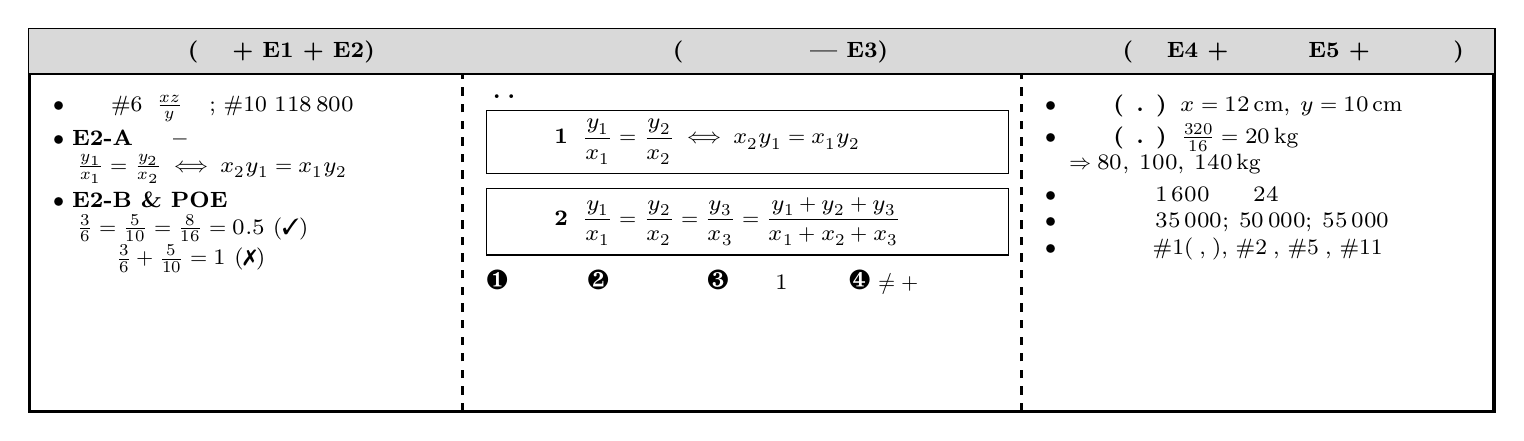
\begin{tikzpicture}[x=1cm, y=1cm, every node/.style={font=\footnotesize, text=black}]
  \draw[black, line width=1.2pt] (0,0) rectangle (18.6,4.85);
  \fill[headgray] (0,4.28) rectangle (18.6,4.85);
  \draw[black, line width=0.8pt] (0,4.28) -- (18.6,4.28);
  \draw[black, line width=0.85pt, dashed] (5.5,0) -- (5.5,4.28);
  \draw[black, line width=0.85pt, dashed] (12.6,0) -- (12.6,4.28);

  \node at (2.75,4.56) {\textbf{ផ្នែកឆ្វេង (កំណែ + \en{E1} + \en{E2})}};
  \node at (9.05,4.56) {\textbf{ផ្នែកកណ្ដាល (ខ្លឹមសារគោលរក្សាទុក — \en{E3})}};
  \node at (15.6,4.56) {\textbf{ផ្នែកស្ដាំ (គំរូ \en{E4} + ប្រតិបត្តិ \en{E5} + កិច្ចការផ្ទះ)}};

  \node[anchor=north west, align=left] at (0.18,4.14) {
    $\bullet$ \textbf{កំណែ៖} \#6គ $\frac{xz}{y}$ រៀល; \#10 $118\,800\riel$\\[2pt]
    $\bullet$ \textbf{\en{E2-A} តួចុង–តួមធ្យម៖}\\
    \hspace*{0.3cm}$\frac{y_1}{x_1}=\frac{y_2}{x_2} \iff x_2 y_1 = x_1 y_2$\\[2pt]
    $\bullet$ \textbf{\en{E2-B} \& \en{POE}៖}\\
    \hspace*{0.3cm}$\frac{3}{6}=\frac{5}{10}=\frac{8}{16}=0.5$ (\ding{51})\\
    \hspace*{0.3cm}ខុសពី $\frac{3}{6}+\frac{5}{10}=1$ (\ding{55})
  };

  \node[anchor=north west, align=left] at (5.68,4.14) {
    {\muol\fontsize{8.4pt}{12pt}\selectfont ១\enbf{.}២\enbf{.} លក្ខណៈនៃសមាមាត្រស្រប}\\[3pt]
    \fbox{\parbox{6.4cm}{\textbf{លក្ខណៈទី 1៖} $\dfrac{y_1}{x_1}=\dfrac{y_2}{x_2} \iff x_2 y_1 = x_1 y_2$}}\\[4pt]
    \fbox{\parbox{6.4cm}{\textbf{លក្ខណៈទី 2៖} $\dfrac{y_1}{x_1}=\dfrac{y_2}{x_2}=\dfrac{y_3}{x_3}=\dfrac{y_1+y_2+y_3}{x_1+x_2+x_3}$}}\\[4pt]
    \cnum{1} គុណខ្វែង \; \cnum{2} តម្រៀបខ្នាត \; \cnum{3} តម្លៃ $1$ ចំណែក \; \cnum{4} $\neq +$
  };

  \node[anchor=north west, align=left] at (12.78,4.14) {
    $\bullet$ \textbf{គំរូ ១ (ទំ.២៩)៖} $x=12\unit{cm},\; y=10\unit{cm}$\\[2pt]
    $\bullet$ \textbf{គំរូ ២ (ទំ.៣០)៖} $\frac{320}{16}=20\unit{kg}$\\
    \hspace*{0.3cm}$\Rightarrow 80,\; 100,\; 140\unit{kg}$\\[2pt]
    $\bullet$ \textbf{ប្រតិបត្តិ ១៖} $1\,600\riel$ និង $24$ ផ្លែ\\
    $\bullet$ \textbf{ប្រតិបត្តិ ២៖} $35\,000;\; 50\,000;\; 55\,000\riel$\\
    $\bullet$ \textbf{កិច្ចការផ្ទះ៖} \#1(ក,ខ), \#2ក, \#5ក, \#11
  };
\end{tikzpicture}
\end{center}

\secstrip{២. ចម្លើយផ្ទៀងផ្ទាត់រហ័សសម្រាប់សន្លឹកកិច្ចការសិស្ស (ទំព័រ ១ និង ទំព័រ ២)}{\en{Answer Key}}

\begin{tcolorbox}[
  enhanced, sharp corners, colback=white, colframe=black,
  boxrule=0.8pt, boxsep=1.5pt, top=3pt, bottom=3pt, left=5pt, right=5pt,
  after skip=3.5pt
]
  \fontsize{8.8pt}{13.2pt}\selectfont
  $\bullet$ \textbf{ផ្នែក \en{E1}៖} បញ្ហាទី ១៖ $x = \mathbf{12\unit{cm}}$; បញ្ហាទី ២៖ ចែកនឹង\textbf{មនុស្សសរុប $16$ នាក់} ។\\[2pt]
  $\bullet$ \textbf{ផ្នែក \en{E2}៖} \textbf{សកម្មភាព ១៖} $y_1\cdot \mathbf{x_2} = y_2\cdot \mathbf{x_1}$; $6\times 6 = \mathbf{36}$ និង $4\times 9 = \mathbf{36}$ ។ \textbf{សកម្មភាព ២៖} $\frac{a(x_1+x_2)}{x_1+x_2} = \mathbf{a} \implies \mathbf{\frac{y_1+y_2}{x_1+x_2}}$ (កែសញ្ញា `$-$' លើសៀវភៅទំ.២៩ មកជា `$=$') ។ \en{POE}៖ $\frac{8}{16} = \mathbf{0.5}$ (\textbf{ស្មើ}); ចំពោះផលបូកគឺ $\mathbf{1} \neq \frac{8}{16}$ (ហាមប្រើលើសញ្ញា $\mathbf{+}$) ។\\[2pt]
  $\bullet$ \textbf{ផ្នែក \en{E4}៖} \textbf{គំរូ ១៖} ក) $2x = 24 \implies x = \mathbf{12\unit{cm}}$; ខ) $3y = 30 \implies y = \mathbf{10\unit{cm}}$ ។ \textbf{គំរូ ២៖} $\frac{320}{16} = \mathbf{20}\unit{kg}/\text{នាក់} \implies a=\mathbf{80\unit{kg}}, b=\mathbf{100\unit{kg}}, c=\mathbf{140\unit{kg}}$ (ផ្ទៀង៖ $80+100+140 = 320\unit{kg}$) ។\\[2pt]
  $\bullet$ \textbf{ផ្នែក \en{E5}៖} \textbf{១) ផ្លែក្រូច៖} ក) $y = \mathbf{1\,600\riel}$; ខ) $x = \mathbf{24}$ ផ្លែ ។ \textbf{២) ចែកប្រាក់៖} $\frac{140\,000}{28} = \mathbf{5\,000\riel/\text{ឆ្នាំ}} \implies a = \mathbf{35\,000\riel},\; b = \mathbf{50\,000\riel},\; c = \mathbf{55\,000\riel}$ ។ \textbf{៣) វិនិច្ឆ័យ \en{A--D}៖} ជម្រើស \textbf{\en{B}} ។ \textbf{៤) សំបុត្រចេញ៖} (ក) $x = \mathbf{10}$; (ខ) $a = \mathbf{14},\; b = \mathbf{21}$ ។
\end{tcolorbox}

\secstrip{៣. ចម្លើយលម្អិតនៃកិច្ចការផ្ទះ (សម្រាប់ផ្ទៀងនៅដើមម៉ោងបន្ទាប់ ១.៣)}{សៀវភៅគោល ទំ.៤០--៤១}

\begin{tcolorbox}[
  enhanced, sharp corners, colback=panelgray, colframe=black,
  boxrule=0.85pt, boxsep=1.5pt, top=3pt, bottom=3pt, left=5pt, right=5pt
]
  \fontsize{8.8pt}{13.2pt}\selectfont
  $\bullet$ \textbf{\#1 ក, ខ (ទំ.៤០)៖} ក) $\dfrac{4}{7} = \dfrac{x}{5} \implies 7x = 20 \implies x = \mathbf{\dfrac{20}{7}}$ ។ \quad ខ) $\dfrac{x}{8} = \dfrac{99}{5} \implies 5x = 792 \implies x = \mathbf{\dfrac{792}{5}} = 158.4$ ។\\[2pt]
  $\bullet$ \textbf{\#2 ក (ទំ.៤០)៖} $\dfrac{a}{5} = \dfrac{b}{18} = \dfrac{a+b}{5+18} = \dfrac{138}{23} = 6 \implies b = 18\times 6 = \mathbf{108}$ (និង $a = 30$) ។\\[2pt]
  $\bullet$ \textbf{\#5 ក (ទំ.៤០)៖} $\dfrac{a}{7} = \dfrac{b}{13} = \dfrac{c}{20} = \dfrac{520}{7+13+20} = \dfrac{520}{40} = 13\riel \implies a = \mathbf{91\riel},\; b = \mathbf{169\riel},\; c = \mathbf{260\riel}$ ។\\[2pt]
  $\bullet$ \textbf{\#11 (ទំ.៤១)៖} តាងចំណែក $A, B, C$ សមាមាត្រនឹង $14, 16, 18$៖ $\dfrac{A}{14} = \dfrac{B}{16} = \dfrac{C}{18}$ ។ ដោយ $A = 105\,000\riel \implies$ តម្លៃ $1$ ចំណែក $= \dfrac{105\,000}{14} = \mathbf{7\,500\riel/\text{ឆ្នាំ}}$ ។ ដូច្នេះ $B = 16\times 7\,500 = \mathbf{120\,000\riel}$, $C = 18\times 7\,500 = \mathbf{135\,000\riel}$ និងប្រាក់សរុប $= (14+16+18)\times 7\,500 = 48\times 7\,500 = \mathbf{360\,000\riel}$ ។
\end{tcolorbox}

\end{document}
